\documentclass[12pt]{article}

% =====================================================================
%  RAPPORT PRBE 2026 — Simulation du mouvement humain et interaction
%  homme-robot dans RoboDK (sujet #47, ligne ALIX, ISAE-SUPMECA)
%  Preambule repris du template ecole (cahier des charges) + ajouts.
%  Rapport monolithique : tout le contenu est dans ce seul fichier.
% =====================================================================

% PACKAGES FOR TITLES
\usepackage{titlesec}
\usepackage{xcolor}
\definecolor{supmerange}{rgb}{0.95,0.07,0.13}

% PACKAGES FOR LANGUAGE AND FONT
\usepackage[utf8]{inputenc}
\usepackage[french]{babel}
\usepackage[T1]{fontenc}
\usepackage{geometry}
\geometry{
  top=2.5cm, left=2.54cm, right=2.54cm, bottom=2.54cm,
  headheight=2cm, headsep=0cm,
}
\usepackage{setspace}

% PACKAGES FOR IMAGES
\usepackage{graphicx}
\graphicspath{{figures/}{Images/}{Page_Garde/}}
\usepackage{float}        % pour [H]
\usepackage{eso-pic}
\usepackage{subfig}
\usepackage{caption}
\usepackage{transparent}
\usepackage{tikz}
\usetikzlibrary{shapes.geometric, arrows.meta, positioning, calc}

% STANDARD MATH PACKAGES
\usepackage{amsmath}
\usepackage{amsthm}
\usepackage{bm}
\usepackage[overload]{empheq}

% PACKAGES FOR TABLES
\usepackage{tabularx}
\usepackage{longtable}
\usepackage{colortbl}
\usepackage{booktabs}
\usepackage{diagbox}

% REFERENCES & BIBLIOGRAPHY
\usepackage[colorlinks=true,linkcolor=black,anchorcolor=black,citecolor=black,filecolor=black,menucolor=black,runcolor=black,urlcolor=black]{hyperref}
\usepackage{cleveref}
\usepackage[square, numbers, sort&compress]{natbib}
\bibliographystyle{plainnat}

% APPENDIX / LISTS / MISC
\usepackage{appendix}
\usepackage{enumitem}
\usepackage{thmtools}
\usepackage{fancyhdr}
\usepackage{tcolorbox}
\usepackage{stfloats}

% ---- Commandes utilitaires ----
\newcommand{\mytitle}[1]{\paragraph*{#1}\mbox{}\par\noindent}
\renewcommand{\figurename}{\textcolor{supmerange}{Figure}}
\renewcommand{\tablename}{\textcolor{supmerange}{Tableau}}

% Barre rouge pleine largeur (identite ISAE du template)
\newcommand{\barre}{\noindent\textcolor{supmerange}{\rule{\textwidth}{3pt}}}
% Section encadree par deux barres rouges (style du template)
\newcommand{\rsection}[1]{%
  \barre\par\vspace{2pt}%
  \section{#1}%
  \vspace{-6pt}\barre\par\vspace{0.7em}}

% ---- En-tete / pied de page ----
\pagestyle{fancy}
\fancyhf{}
\fancyhead[C]{\textcolor{supmerange}{Simulation du mouvement humain et interaction homme-robot dans RoboDK}}
\fancyfoot[L]{\textcolor{supmerange}{ISAE-SUPMECA | Formation d'ingénieur Statut Étudiant}}
\fancyfoot[R]{\textcolor{supmerange}{\thepage}}
\renewcommand{\headrulewidth}{0pt}
\setlength{\headsep}{25pt}

\title{Simulation du mouvement humain et interaction homme-robot dans RoboDK}
\author{Niko Khachidze, Alexandre Nowak, Luc Fantasia}
\date{2026}

\begin{document}

% ====================== PAGE DE GARDE ======================
\newcommand\BackgroundPic{%
  \put(0,0){%
    \parbox[b][\paperheight]{\paperwidth}{%
      \vfill\centering
      
\includegraphics[height=\paperheight]{Page_Garde/PremierePage.png}%
      \vfill}}}

\begin{titlepage}
  \thispagestyle{empty}
  \AddToShipoutPicture*{\BackgroundPic}
  \vspace*{\fill}
  \begin{center}
  \colorbox{white}{%
  \begin{minipage}[c][17.5cm][c]{0.75\textwidth}
    \centering
    \setstretch{2}
    {\Huge\bfseries Simulation du mouvement humain et interaction homme-robot dans RoboDK}\\
    \vspace{0.5em}
    {\Large \bfseries Rapport de projet --- PRBE Homme-Robot}\\
    \vspace{0.5em}
    {\Large ISAE-SUPMÉCA}\\
    \textcolor{supmerange}{\rule{0.1\textwidth}{3pt}}\\
    30 rue Fernand Hainaut, 93400 Saint-Ouen-sur-Seine\\
    Niko Khachidze, Alexandre Nowak, Luc Fantasia\\
    \textit{Encadrants : Francesco Ciampi, Thierno Diallo}\\
    \textcolor{supmerange}{\rule{0.1\textwidth}{3pt}}\\
    {\normalsize Avril 2026 -- Juin 2026}\\
    
\includegraphics[width=0.5\textwidth]{Page_Garde/logo_isae-supmeca.png}
  \end{minipage}}
  \end{center}
\end{titlepage}

\newpage
\tableofcontents
\newpage

% ====================== CORPS DU RAPPORT ======================
% Repartition : Niko = sections 4 (modele conceptuel, partie RoboDK),
% 5 (developpement), 6 (tests & resultats), 7 (conclusion).
% Alex / Luc = contexte, cahier des charges, etat de l'art,
% cinematique formelle (placeholders ci-dessous a raccorder).

% =====================================================================
% SECTION 1 — CONTEXTE ET OBJECTIFS
% Responsable : Alex / Luc (partie commune). Base reprise du cahier des
% charges de l'equipe. >>> A VALIDER / COMPLETER par Alex & Luc <<<
% =====================================================================

\rsection{Contexte et objectifs du projet}

Le projet porte sur la simulation d'interactions entre un opérateur humain et un
robot manipulateur mobile dans l'environnement \textsc{RoboDK}, en s'appuyant sur
la ligne \textbf{ALIX} de l'ISAE-SUPMÉCA.
Cette ligne est un système de production cyber-physique sur lequel circulent des
pièces, qu'un bras robotisé récupère et qu'un opérateur humain manipule.

\medskip
\noindent\textbf{Problématique.}
Dans les environnements industriels collaboratifs, robots et opérateurs partagent
le même espace de travail. Concevoir et valider ces interactions est un enjeu de
\emph{sécurité}, d'\emph{ergonomie} et d'\emph{efficacité}. Les outils de
simulation modélisent finement les robots, mais la représentation réaliste du
\textbf{mouvement humain} et de son interaction dynamique avec les robots reste
un verrou : \textsc{RoboDK} ne propose pas de modèle humain cinématique pilotable.
Le projet vise donc à \textbf{construire le pont} entre un mannequin humain et la
simulation robotique.

\medskip
\noindent\textbf{Objectif principal.}
Représenter dans \textsc{RoboDK} un opérateur articulé, le faire se déplacer et
manipuler des pièces, puis simuler des scénarios d'interaction homme-robot afin
d'évaluer les conditions de sécurité et d'organisation du travail.

\medskip
\noindent\textbf{Objectifs détaillés.}
\begin{itemize}[noitemsep]
  \item développer un modèle cinématique simplifié d'un mannequin adapté à la simulation ;
  \item implémenter la génération des mouvements des membres inférieurs (locomotion) ;
  \item implémenter la génération des mouvements des membres supérieurs (manipulation) ;
  \item simuler des scénarios d'interaction homme-robot ;
  \item analyser ces interactions pour identifier des contraintes de sécurité et d'ergonomie.
\end{itemize}

% >>> Alex/Luc : completer/ajuster ce contexte, ajouter eventuellement
%     un schema de la ligne ALIX et une photo du poste etudie. <<<

% =====================================================================
% SECTION 2 - CAHIER DES CHARGES
% Responsable : Alex / Luc. Le cahier des charges complet existe deja
% (docs/cahier-des-charges.md + PDF 17 p). >>> A CONDENSER en ~2 pages
% par Alex & Luc, ou a reprendre depuis leur version LaTeX. <<<
% Trame minimale ci-dessous pour que le document compile.
% =====================================================================

\rsection{Cahier des charges}

Cette section résume le cahier des charges du projet. Sa version complète est
donnée en annexe (\cref{annexe:cdc}) et maintenue sur le dépôt GitHub du projet.

\subsection{Scénarios étudiés}
Les deux scénarios sont résumés ci-dessous ; leur description complète figure en
annexe (\cref{annexe:cdc}).

\paragraph{Scénario 1 --- Coexistence.} Robot et opérateur partagent la zone sans
interaction directe ni indirecte. Règles de sécurité : ralentissement à 1~m,
arrêt à 0{,}5~m ; logique de porte (arrêt si présence, recul après 30~s si
l'humain reste immobile, reprise sinon).

\paragraph{Scénario 2 --- Synchronisation.} Robot et opérateur travaillent sur la
même ligne avec interaction \emph{indirecte} : le robot dépose des lots de pièces
sur une plateforme tampon, l'opérateur les assemble. La passation est pilotée par
des \textbf{déclencheurs} (signaux sonores/lumineux).

\subsection{Exigences fonctionnelles (extrait)}
La liste complète des exigences fonctionnelles figure en annexe
(\cref{annexe:cdc}).
\begin{itemize}[noitemsep]
  \item \textbf{EF1} --- le mannequin articulé est simulé dans \textsc{RoboDK} et piloté en Python ;
  \item \textbf{EF2} --- il réalise des mouvements simples des membres supérieurs et inférieurs ;
  \item \textbf{EF3} --- animation synchronisée du mannequin et du robot ;
  \item \textbf{EF4--EF6} --- détection de proximité, ralentissement/arrêt, distance minimale.
\end{itemize}

\subsection{Périmètre et limites}
Le mannequin reste \textbf{simplifié} (compromis réalisme / complexité
cinématique). On vise des mouvements visuellement cohérents, sans reproduction
biomécanique complète. Hors périmètre : équilibre dynamique, contact physique
direct, capture caméra temps réel. Le modèle retenu compte \textbf{22 degrés de
liberté} (cf. \cref{sec:modele}). Le détail du périmètre et des limites figure
dans le cahier des charges complet (\cref{annexe:cdc}).

% >>> Inserer ici le diagramme de Gantt et le tableau d'affectation des taches. <<<

% =====================================================================
% SECTION 3 --- ETAT DE L'ART
% Responsable : Alex / Luc. Base : docs/etat-de-l-art.md + analyse
% bibliographique (4 papiers). >>> A REDIGER sous forme argumentee
% (applicable / non + justification), pas exhaustive. <<<
% =====================================================================

\rsection{État de l'art}

Trois familles d'approches existent pour animer un modèle humain en simulation :
\begin{enumerate}[noitemsep]
  \item \textbf{analytique} (animation par points / poses clés) ;
  \item \textbf{apprentissage} (bases de données de mouvements, modèles type SMPL) --- jugée trop lourde à mettre en \oe uvre dans notre cadre ;
  \item \textbf{cinématique inverse (IK)} --- approche \textbf{retenue}, combinée à des poses clés.
\end{enumerate}

\medskip
\noindent\textbf{Sources principales.}
\begin{itemize}[noitemsep]
  \item \emph{Human Model Generator} (HMG, IIT) --- générateur de mannequin URDF
        anthropométrique scalable ; base de notre modèle~\cite{hmg}.
  \item Latella \emph{et al.} 2019 --- spécification du modèle 23~liens / 48~DDL
        qui alimente le HMG~\cite{latella2019}.
  \item Kim \emph{et al.} 2009 --- pipeline \emph{motion capture} $\rightarrow$
        mouvements articulaires, IK des membres inférieurs~\cite{kim2009}.
  \item Maurice \emph{et al.} 2019 --- \emph{Digital Human Modeling} pour la
        robotique collaborative, indicateurs ergonomiques~\cite{maurice2019}.
  \item Tola \& Corke 2023 --- confirme l'absence de support URDF natif dans
        plusieurs simulateurs et la nécessité d'une conversion~\cite{tola2023}.
\end{itemize}

\medskip
\noindent\textbf{Cadre normatif (sécurité).} ISO~10218-1/2 (robots
industriels)~\cite{iso10218}, ISO/TS~15066 (robotique
collaborative)~\cite{isots15066}, ISO~13857 (distances de sécurité). Ces normes
fixent les distances et conditions d'arrêt mobilisées dans les scénarios.

% >>> Alex/Luc : developper chaque source (1 paragraphe applicable/non). <<<

% =====================================================================
% SECTION 4 --- MODELE CONCEPTUEL                          [NIKO + Alex]
% 4.1 schema cinematique / DDL (formel : Alex) ; 4.2 demarche de
% developpement (Niko) ; 4.3 arborescence des reperes (Niko).
% =====================================================================

\rsection{Modèle conceptuel}
\label{sec:modele}

Le modèle conceptuel répond à une question : \emph{comment représenter un
opérateur humain articulé, pilotable, à l'intérieur de \textsc{RoboDK}} ? On le
décrit en trois temps : la base \textbf{cinématique} (liaisons et degrés de
liberté), la \textbf{démarche de développement} (du modèle figé à l'opérateur
animé) et l'\textbf{arborescence des repères} qui matérialise l'articulation
dans le logiciel.

% ---------------------------------------------------------------
\subsection{Schéma cinématique et degrés de liberté}
\label{ssec:cinematique}

Le corps est modélisé comme un \textbf{arbre de solides rigides} reliés par des
liaisons normalisées. Le tronc (épine, cou, tête, clavicules)
est traité comme un \emph{unique solide rigide} : ses articulations sont des
encastrements. Les membres portent les degrés de liberté.

\begin{table}[H]
\centering
\caption{Liaisons normalisées du modèle et degrés de liberté associés.}
\label{tab:liaisons}
\begin{tabular}{@{}llc@{}}
\toprule
\textbf{Articulation} & \textbf{Liaison normalisée} & \textbf{DDL} \\
\midrule
Épaule, hanche & Rotule & 3 rotations \\
Coude, genou, cheville & Pivot & 1 rotation \\
Poignet & Rotule à doigt & 2 rotations \\
Tronc (épine, cou, tête, clavicules) & Encastrement & 0 \\
\bottomrule
\end{tabular}
\end{table}

Chaque liaison se lit sur son \textbf{torseur cinématique} : les composantes de
rotation non nulles sont les degrés de liberté laissés libres. Pour une rotule de
centre $A$, par exemple,
\[
\{\mathcal{V}\}_A=\begin{Bmatrix}\omega_x & 0\\ \omega_y & 0\\ \omega_z & 0\end{Bmatrix}_A ,
\]
soit trois rotations libres et aucune translation. Le bilan global donne
\[
\underbrace{2\,(3+1+2)}_{\text{bras}} \;+\; \underbrace{2\,(3+1+1)}_{\text{jambes}} \;=\; \boxed{22 \text{ DDL}} .
\]

\begin{figure}[H]
  \centering
  \subfloat[Vue de face]{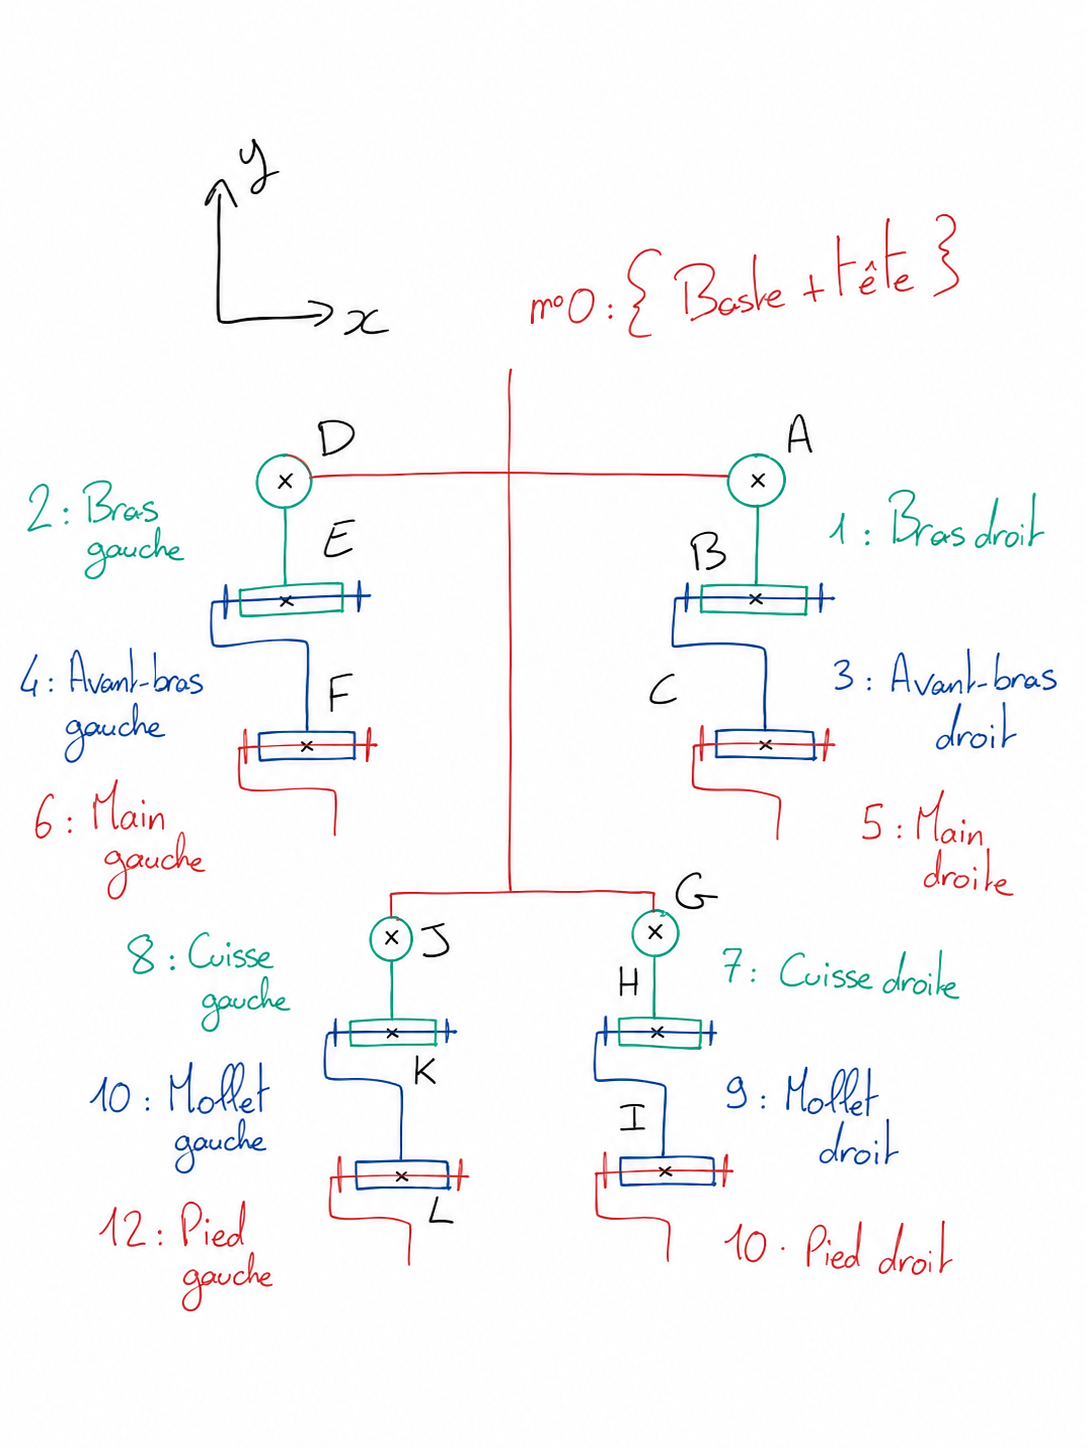
\includegraphics[width=0.42\textwidth]{schema-cinematique-face.png}}\hfil
  \subfloat[Vue de côté]{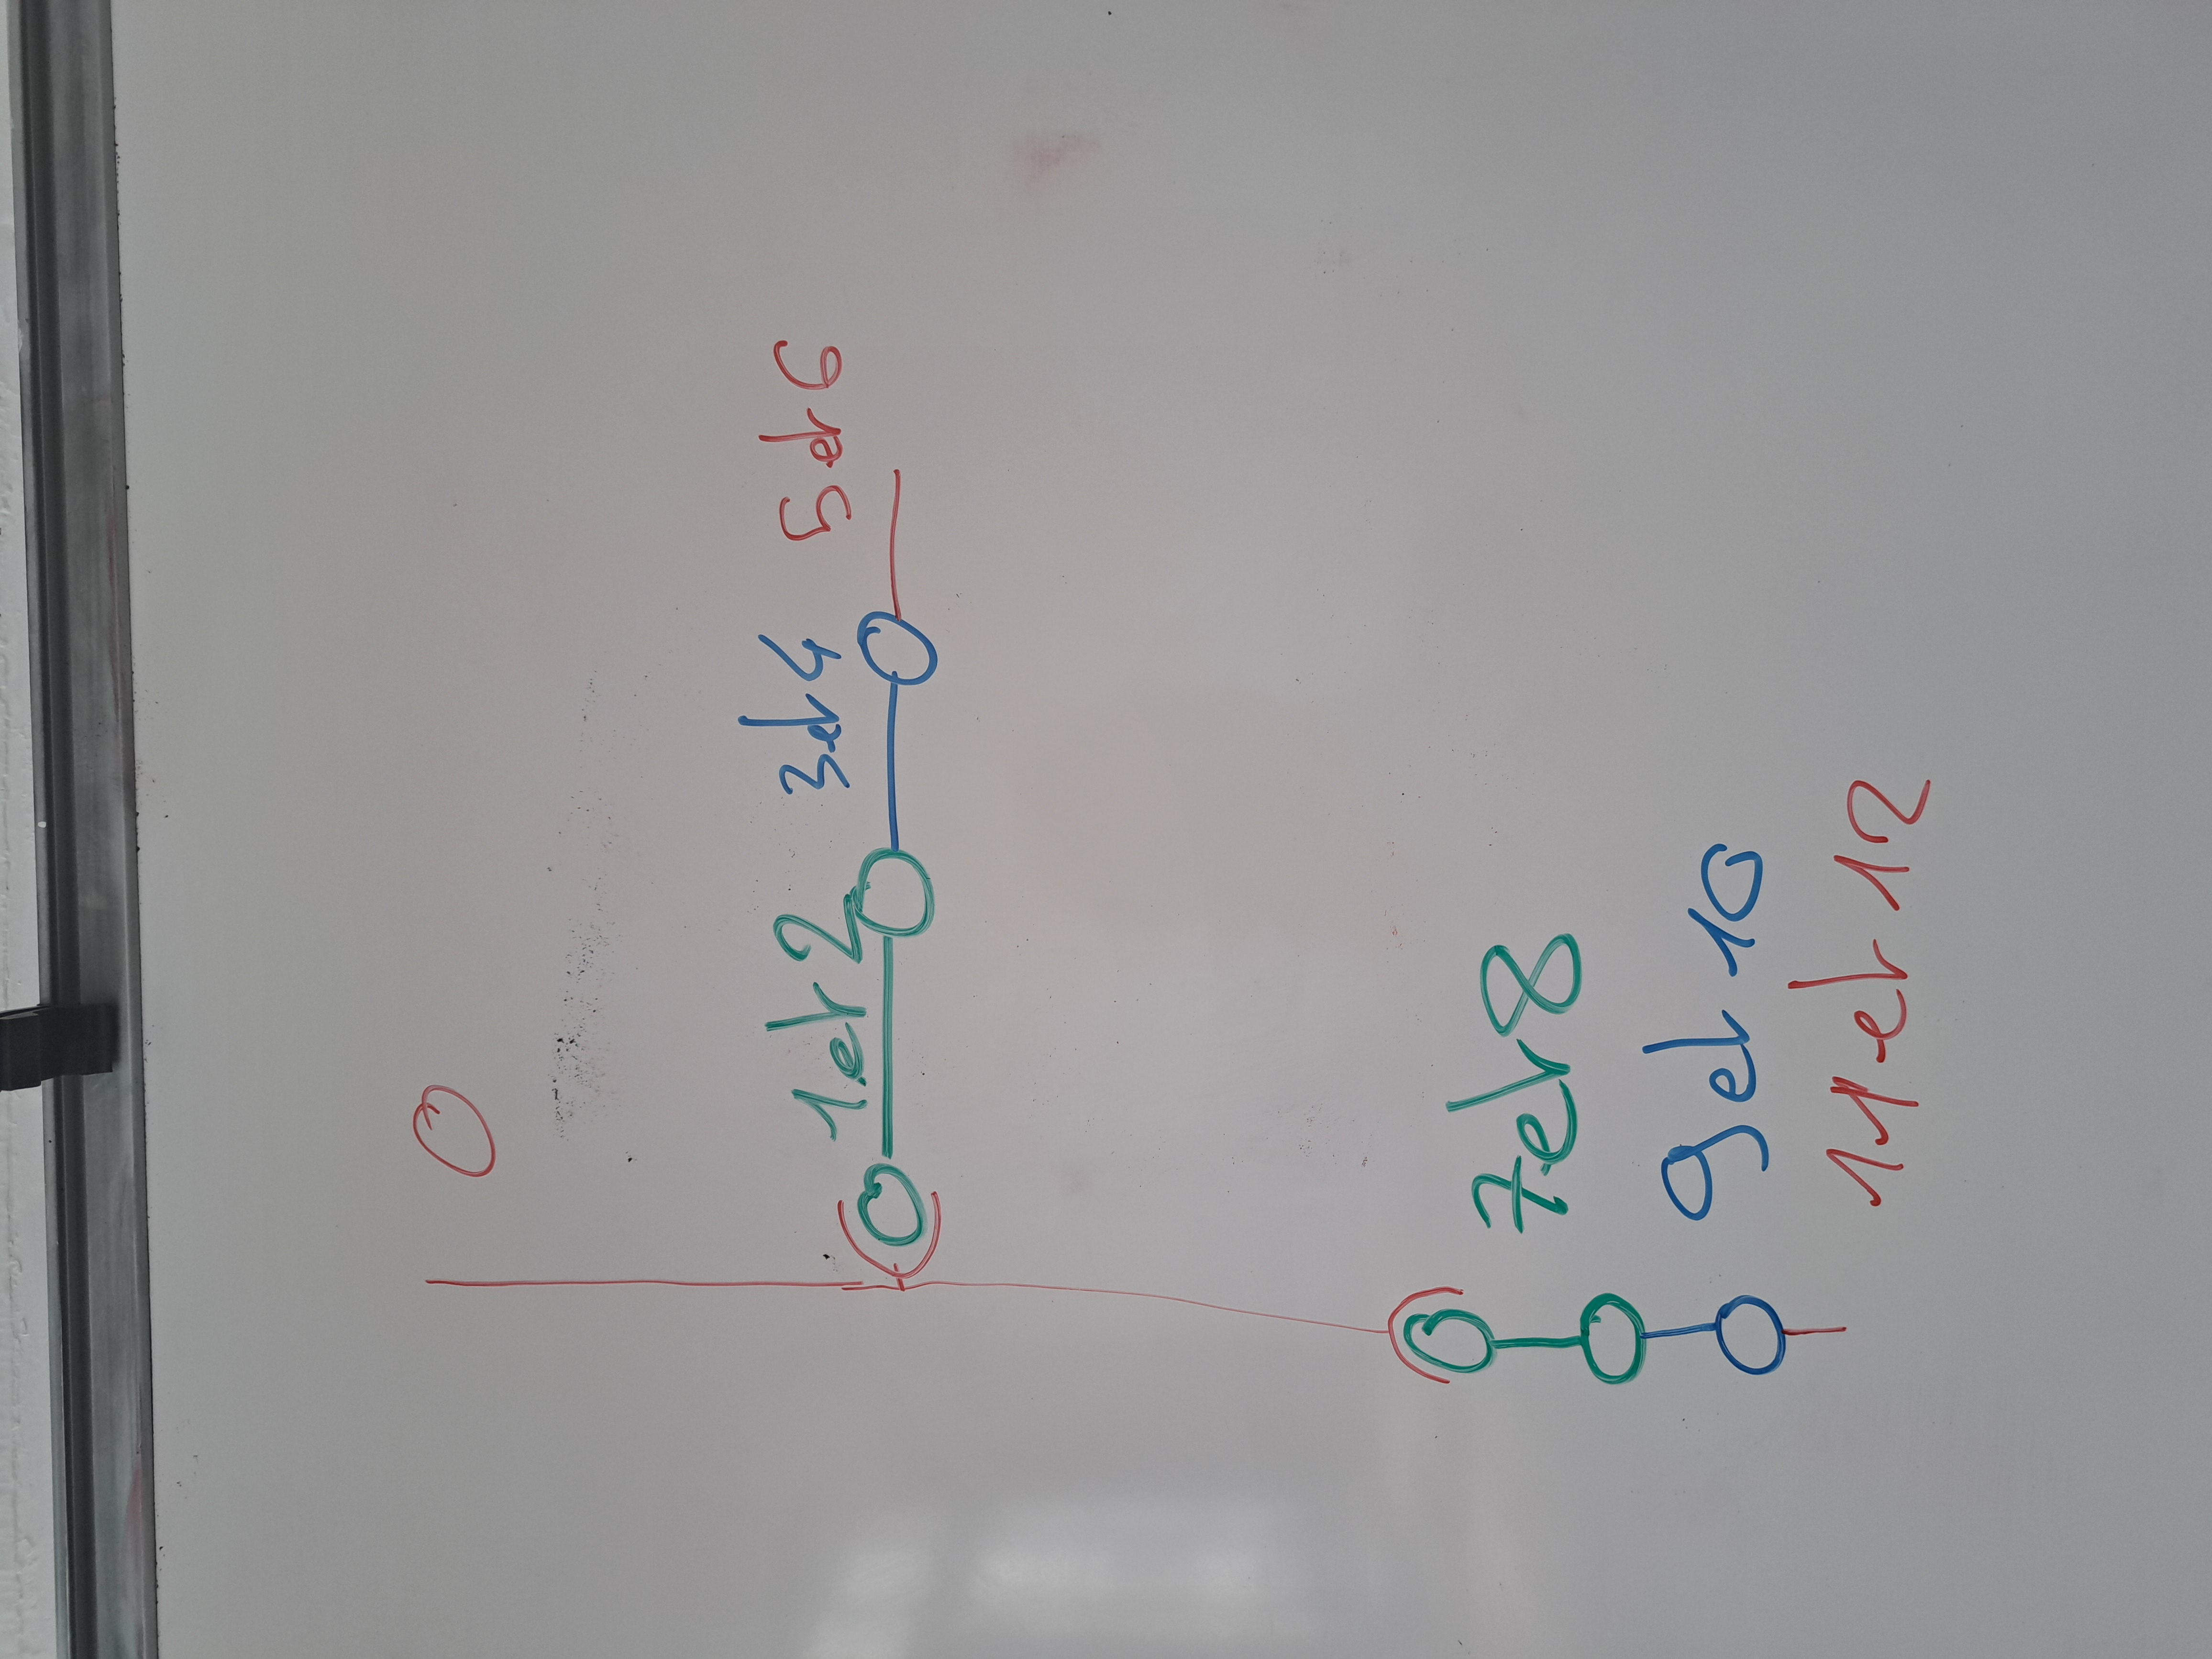
\includegraphics[width=0.42\textwidth]{schema-cinematique-cote.jpg}}
  \caption{Schéma cinématique normalisé du mannequin.}
  \label{fig:schema-cine}
\end{figure}

% ---------------------------------------------------------------
\subsection{Démarche de développement}
\label{ssec:demarche}

Le modèle humain est défini par un fichier \textbf{URDF} généré avec le
\emph{Human Model Generator} (mannequin anthropométrique scalable~: 22~DDL, axes
et butées validés sous iDynTree). Mais \textbf{\textsc{RoboDK} n'importe pas
l'URDF} : son outil \emph{Build Mechanism} ne gère que des chaînes \emph{série}
(7~axes maximum, rotation forcée autour d'un même axe), alors qu'un corps humain
est un \textbf{arbre} de cinq branches issues du tronc.

La stratégie retenue contourne ce verrou (\cref{fig:pipeline}) : on importe le
modèle 3D au format STEP, on le découpe en segments anatomiques, puis on
\emph{reconstruit} l'articulation à la main avec des repères imbriqués et l'API
Python. L'URDF n'est plus un fichier d'import mais une \textbf{table de
référence} (quels DDL, quels axes, quelles butées).

\begin{figure}[H]
\centering
\begin{tikzpicture}[
  node distance=7mm,
  bloc/.style={rectangle, rounded corners, draw=supmerange, very thick,
               fill=supmerange!6, text width=9.2cm, align=center,
               minimum height=0.95cm, font=\small},
  fleche/.style={-{Stealth[length=3mm]}, very thick, draw=supmerange}]
  \node[bloc] (a) {\textbf{Mannequin anthropométrique URDF} (HMG)\\ 22~DDL --- axes et butées de référence};
  \node[bloc, below=of a] (b) {\textbf{Modèle 3D} \texttt{Manikin\_1.STEP}\\ assemblage des segments, déjà positionnés};
  \node[bloc, below=of b] (c) {\textbf{Découpe en segments} (Split)\\ identification \emph{géométrique} des membres};
  \node[bloc, below=of c] (d) {\textbf{Rig à 22 DDL}\\ repères imbriqués + attachement des segments};
  \node[bloc, below=of d] (e) {\textbf{Génération du mouvement}\\ poses clés, marches, manipulation};
  \node[bloc, below=of e] (f) {\textbf{Adaptation à une trajectoire}\\ locomotion guidée par une courbe externe};
  \draw[fleche] (a)--(b); \draw[fleche] (b)--(c); \draw[fleche] (c)--(d);
  \draw[fleche] (d)--(e); \draw[fleche] (e)--(f);
\end{tikzpicture}
\caption{Démarche de développement : du modèle anthropométrique figé à l'opérateur animé sur trajectoire.}
\label{fig:pipeline}
\end{figure}

\paragraph{Découpe et identification.} Le STEP arrive comme \emph{un seul objet}
fusionné. La commande \texttt{Split} le découpe en 17~sous-solides, déjà placés au
bon endroit. Comme leurs noms sont inexploitables, on les identifie
\textbf{par leur position} : le centre de chaque sous-solide est comparé à une
table de 15~ancres anatomiques mesurées une fois sur le modèle, et rattaché à la
plus proche. On obtient 15~segments nommés (bassin, torse, tête, bras, avant-bras,
mains, cuisses, tibias, pieds).

% ---------------------------------------------------------------
\subsection{Arborescence des repères}
\label{ssec:arbo}

Le principe directeur est : \textbf{un repère = un degré de liberté}. Un repère
de \textsc{RoboDK} pourrait tourner librement, mais on s'impose qu'il ne tourne
que sur \emph{un seul} axe. Une articulation à plusieurs DDL (une rotule) est donc
représentée par \textbf{plusieurs repères imbriqués} au même point
(\cref{tab:dof}). La hiérarchie obtenue est un arbre enraciné au bassin
(\cref{fig:arbo}) : quand un repère tourne, tous ses descendants (repères et
segments) suivent --- exactement la cinématique d'un squelette.

\begin{figure}[H]
  \centering
  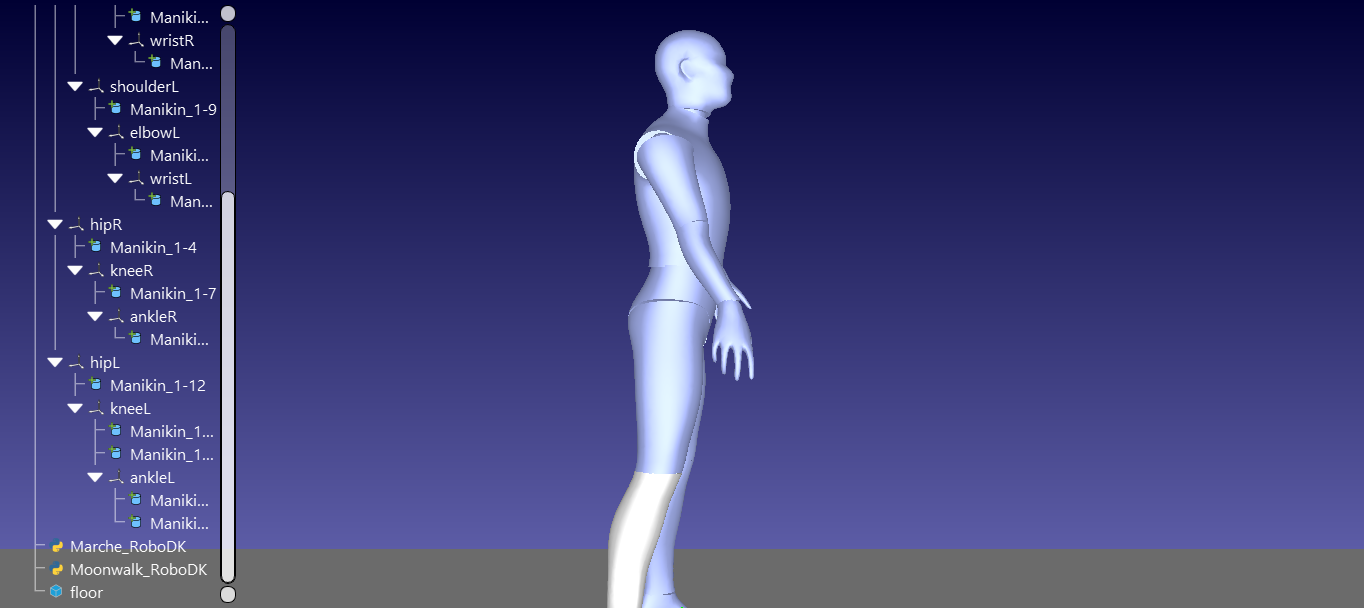
\includegraphics[width=0.9\textwidth]{station_final.png}
  \caption{Opérateur au garde-à-vous dans \textsc{RoboDK} et arborescence des
  repères (panneau de gauche) : \texttt{Human\_Base} $\rightarrow$ hanches /
  épaules $\rightarrow$ genoux / coudes $\rightarrow$ chevilles / poignets.}
  \label{fig:arbo}
\end{figure}

\begin{figure}[H]
\centering
  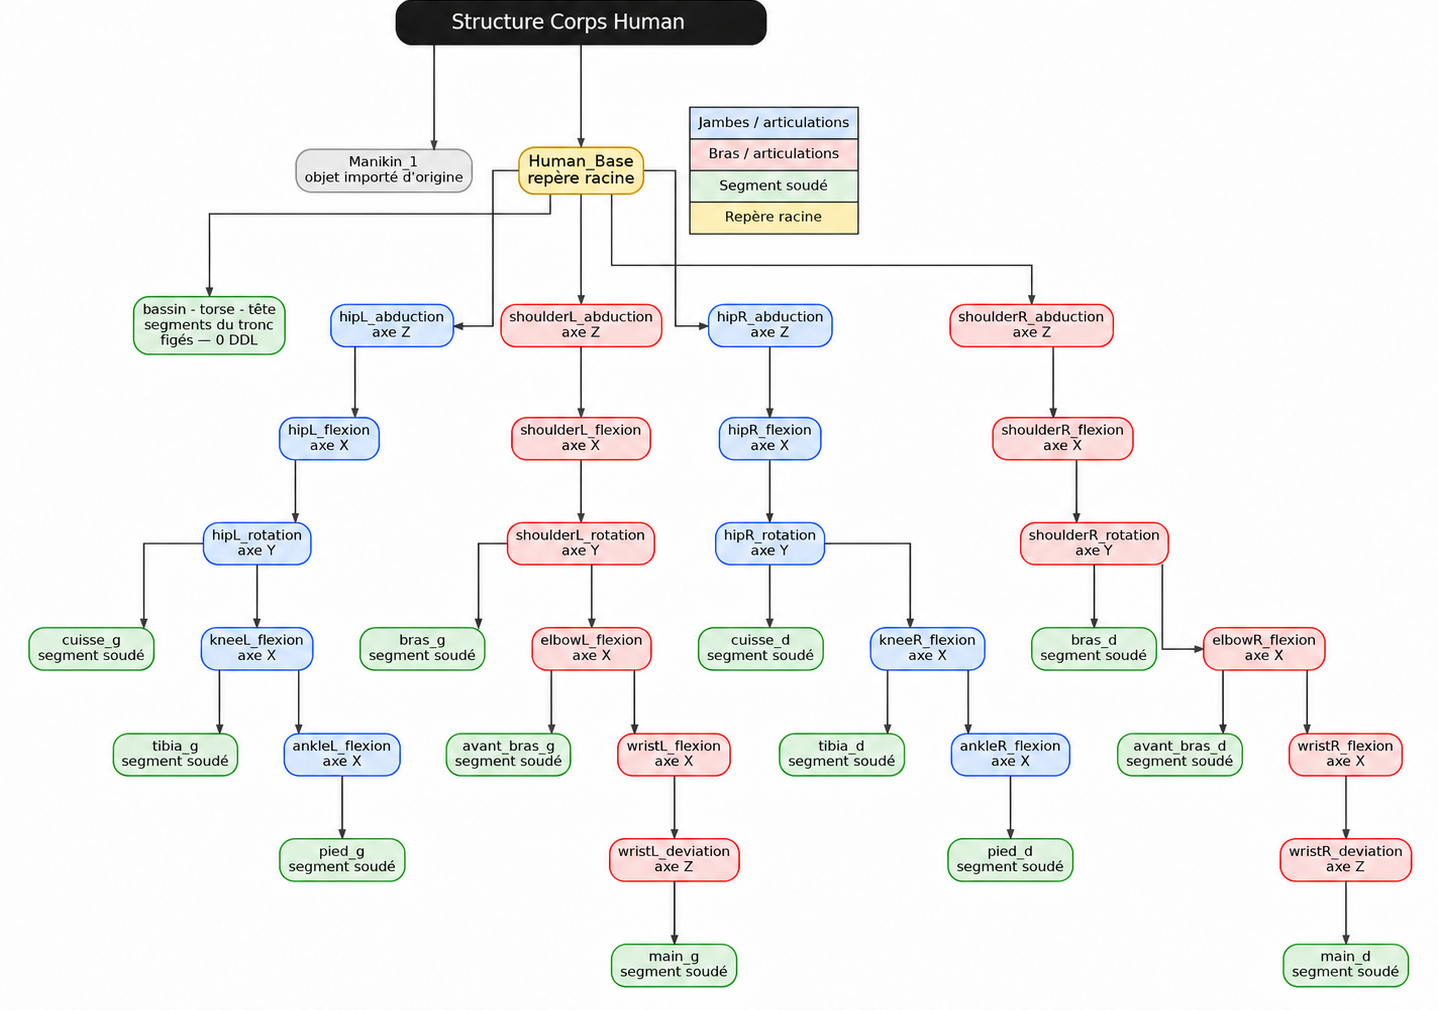
\includegraphics[width=\textwidth]{structure_arborescence.png}
  \caption{Structure de l'arborescence du rig (vue d'ensemble des quatre membres).
  \textbf{Repères} (rouge) : chacun ne porte \emph{qu'un seul} DDL, son axe de
  rotation est indiqué ; une rotule (hanche, épaule) est donc faite de trois
  repères imbriqués --- soit 22~DDL au total. \textbf{Segments de corps} (vert) :
  \emph{soudés} à un repère via \texttt{setParentStatic}, ils n'ont aucun DDL propre
  et suivent toute rotation des repères situés au-dessus d'eux. Le tronc
  (bassin + torse + tête) est encastré sur la racine \texttt{Human\_Base}.}
  \label{fig:arbo-schema}
\end{figure}

\paragraph{Hiérarchie.} Le tronc (bassin + torse + tête) est figé et attaché
directement à la racine \texttt{Human\_Base}. Chaque membre est une chaîne de
repères~:
{\sloppy
\begin{itemize}[noitemsep]
  \item \textbf{Jambe} : \texttt{hip\_abduction} $\to$ \texttt{hip\_flexion}
        $\to$ \texttt{hip\_rotation} $\to$ \texttt{knee\_flexion}
        $\to$ \texttt{ankle\_flexion} ;
  \item \textbf{Bras} : \texttt{shoulder\_abduction} $\to$
        \texttt{shoulder\_flexion} $\to$ \texttt{shoulder\_rotation}
        $\to$ \texttt{elbow\_flexion} $\to$ \texttt{wrist\_flexion}
        $\to$ \texttt{wrist\_deviation}.
\end{itemize}\par}

\paragraph{Placement des repères.} Le centre d'une articulation est pris au
\textbf{centre de la « boule »} qui la matérialise, c'est-à-dire au milieu de
l'intersection des boîtes englobantes des deux segments voisins (la sphère
appartient aux deux). L'épaule fait exception (le torse déborde sur le bras) et
demande un calage manuel.

\paragraph{Convention d'axes.} Le repère monde est orienté \textbf{Y vers le
haut}, \textbf{X vers le côté gauche} du mannequin, \textbf{Z vers l'avant} (le
mannequin regarde vers $+Z$). Les trois mouvements élémentaires sont alors~:
\begin{itemize}[noitemsep]
  \item \textbf{flexion} : rotation autour de $X$ (plan sagittal, avant/arrière) ;
  \item \textbf{abduction} : rotation autour de $Z$ (plan frontal, écarter/serrer) ;
  \item \textbf{rotation} : rotation autour de $Y$ (axe long du membre).
\end{itemize}

\begin{table}[H]
\centering
\caption{Les 22 degrés de liberté et leurs amplitudes (butées URDF, côté droit ;
le côté gauche est le miroir, signes inversés).}
\label{tab:dof}
\small
\begin{tabular}{@{}lllcl@{}}
\toprule
\textbf{Articulation} & \textbf{Liaison} & \textbf{Mouvement} & \textbf{Axe} & \textbf{Amplitude} \\
\midrule
Épaule ($\times 2$) & rotule & abduction & $Z$ & $[-135,\,+90]^\circ$ \\
                    &        & flexion   & $X$ & $[-90,\,+90]^\circ$ \\
                    &        & rotation  & $Y$ & $[-45,\,+180]^\circ$ \\
Coude ($\times 2$)  & pivot  & flexion   & $X$ & $[0,\,+145]^\circ$ \\
Poignet ($\times 2$)& rotule à doigt & flexion & $X$ & $[-50,\,+60]^\circ$ \\
                    &        & déviation & $Z$ & $[-30,\,+20]^\circ$ \\
Hanche ($\times 2$) & rotule & abduction & $Z$ & $[-45,\,+30]^\circ$ \\
                    &        & flexion   & $X$ & $[-120,\,+15]^\circ$ \\
                    &        & rotation  & $Y$ & $[-45,\,+45]^\circ$ \\
Genou ($\times 2$)  & pivot  & flexion   & $X$ & $[0,\,+135]^\circ$ \\
Cheville ($\times 2$)& pivot & flexion   & $X$ & $[-30,\,+50]^\circ$ \\
\bottomrule
\end{tabular}
\end{table}

\begin{figure}[H]
  \centering
  \subfloat[Abduction]{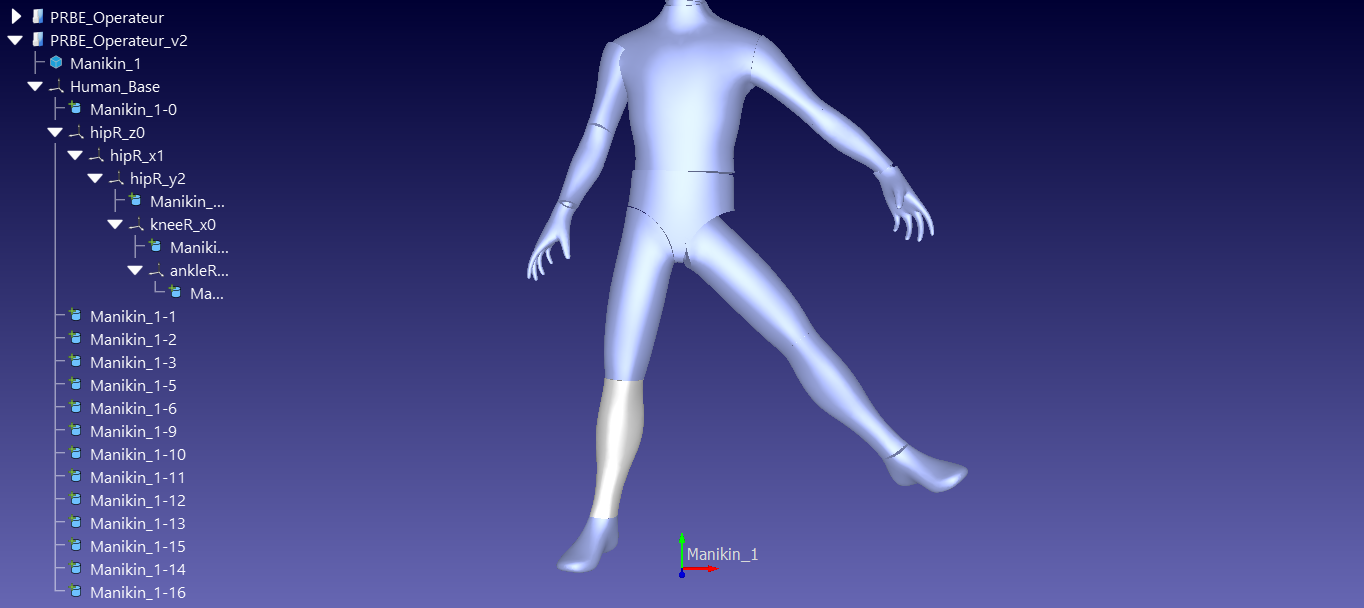
\includegraphics[width=0.31\textwidth]{hip_abduction.png}}\hfil
  \subfloat[Flexion]{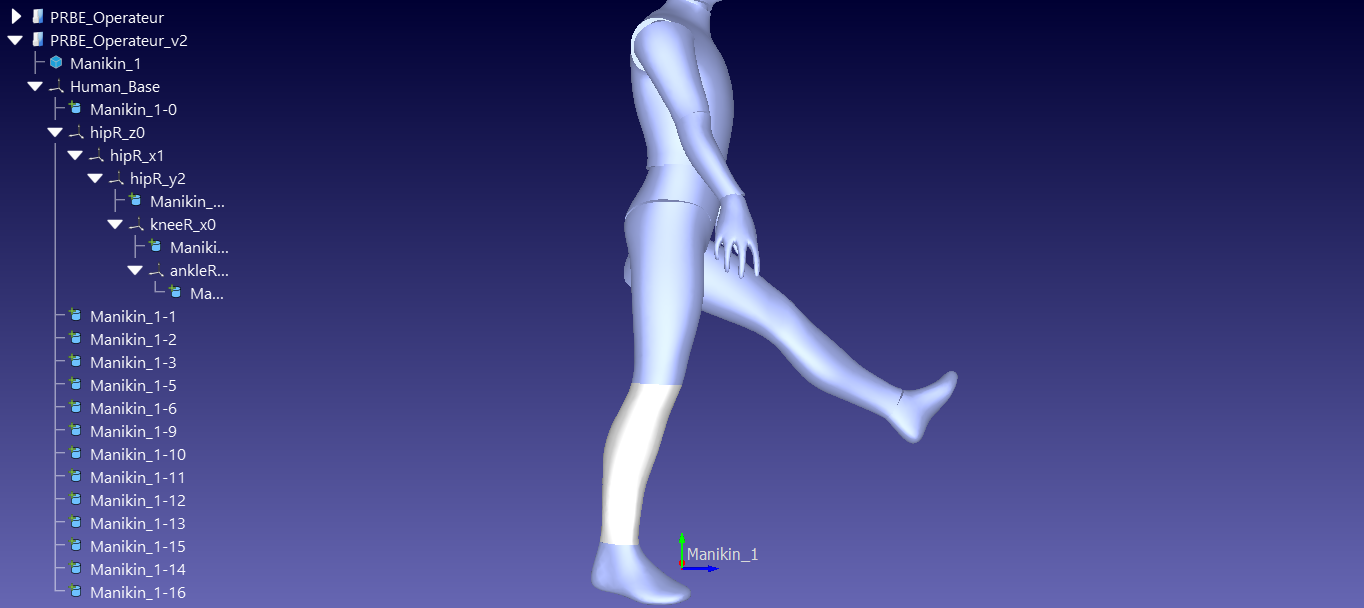
\includegraphics[width=0.31\textwidth]{hip_flexion.png}}\hfil
  \subfloat[Rotation]{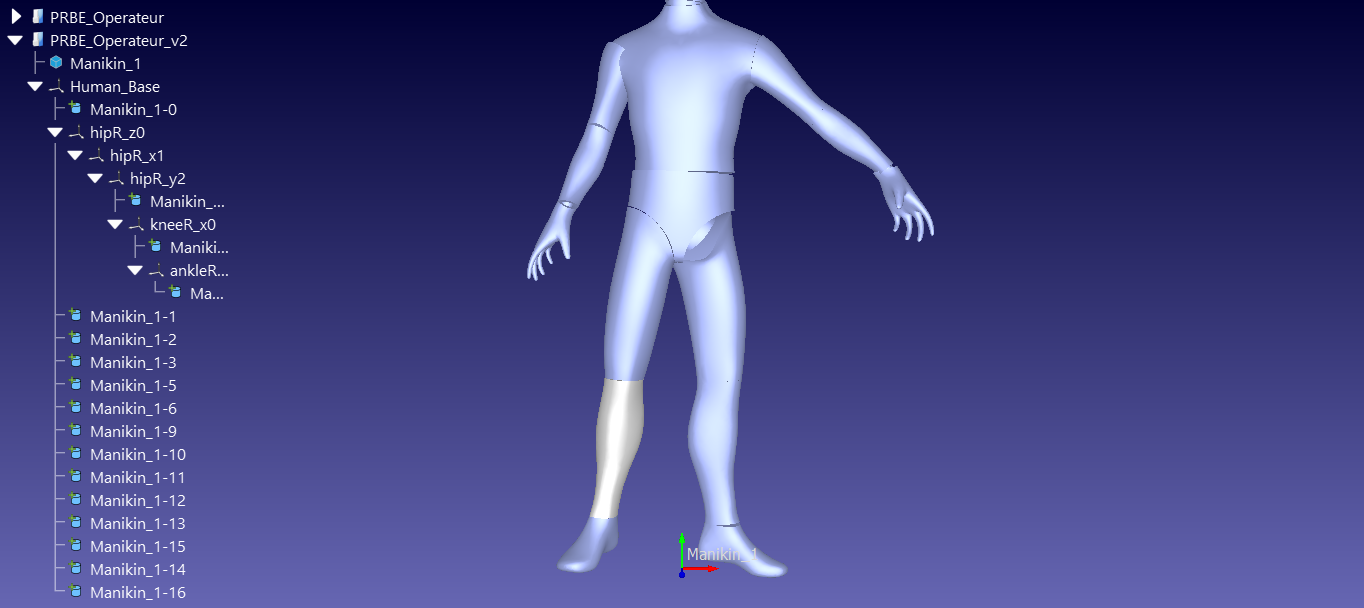
\includegraphics[width=0.31\textwidth]{hip_rotation.png}}
  \caption{Décomposition d'une rotule (hanche) en trois repères imbriqués, chacun
  porteur d'un seul DDL : abduction ($Z$), flexion ($X$), rotation ($Y$).}
  \label{fig:rotule}
\end{figure}

% =====================================================================
% SECTION 5 — DEVELOPPEMENT                                     [NIKO]
% Principe d'animation + locomotion (3 marches) + manipulation (bras).
% Consigne : pas de code brut -> equations et schemas.
% =====================================================================

\rsection{Développement}
\label{sec:dev}

Une fois l'opérateur articulé (\cref{sec:modele}), le développement porte sur la
\textbf{génération du mouvement} : un principe d'animation commun, puis deux
familles de gestes --- la \emph{locomotion} (membres inférieurs) et la
\emph{manipulation} (membres supérieurs).

% ---------------------------------------------------------------
\subsection{Principe d'animation : pose de repos et rotation}
\label{ssec:principe}

Au lancement d'une animation, on \textbf{capture la pose de repos} de chaque
repère (\cref{fig:gav}). Animer un DDL revient à repartir de ce repos et à appliquer une rotation
sur \emph{son} axe, bornée aux butées articulaires~:
\[
F_i(\theta) = R_i^{\text{repos}} \cdot \mathrm{Rot}_{a_i}(\theta),
\qquad \theta \in [\theta_i^{\min},\, \theta_i^{\max}],
\]
où $a_i$ est l'axe du DDL $i$ et $R_i^{\text{repos}}$ sa pose neutre. Cette règle
unique garantit que tout mouvement reste dans les amplitudes physiologiques du
\cref{tab:dof} et que les segments fils suivent leur parent.

\begin{figure}[H]
  \centering
  \subfloat[Face]{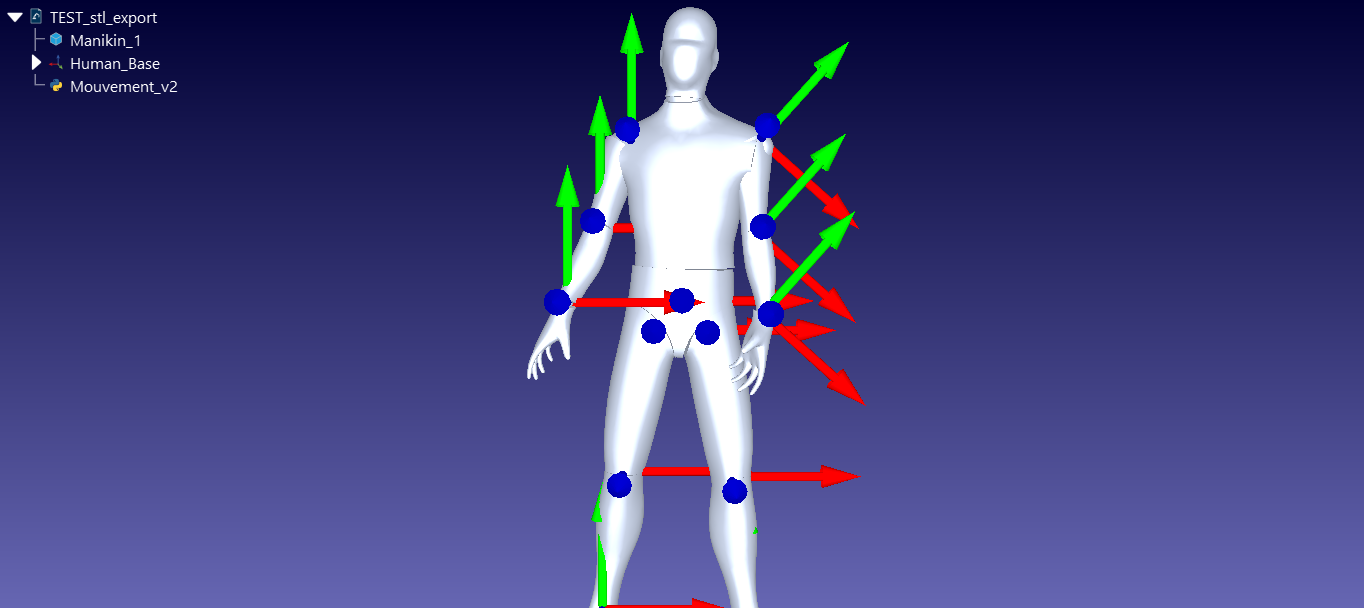
\includegraphics[width=0.3\textwidth]{gav_front.png}}\hfil
  \subfloat[Profil]{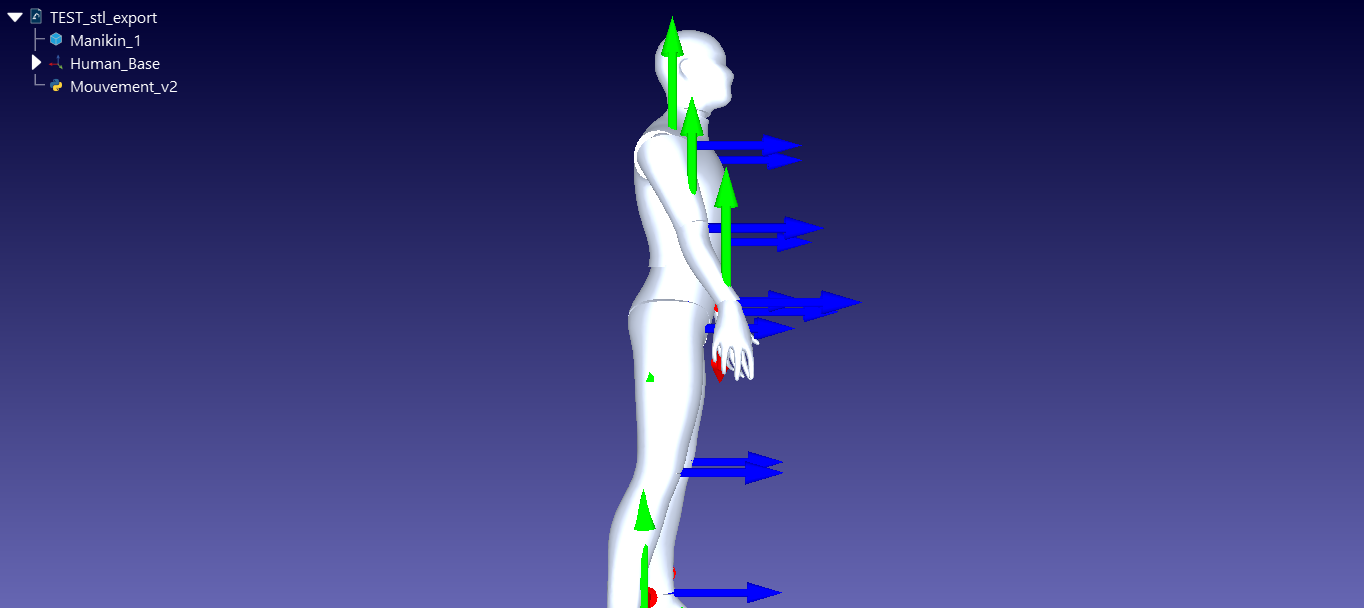
\includegraphics[width=0.3\textwidth]{gav_side.png}}\hfil
  \subfloat[Jambes resserrées]{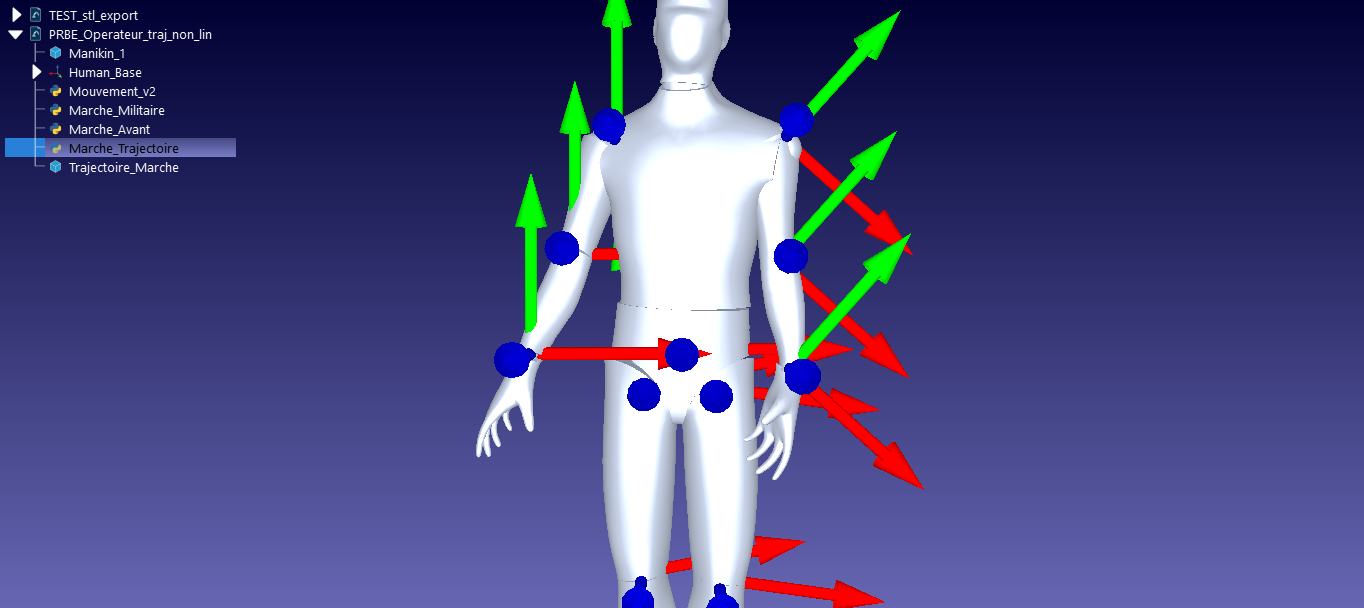
\includegraphics[width=0.3\textwidth]{jambes_resserrees.png}}
  \caption{Pose de repos (garde-à-vous) : référence de toutes les animations.}
  \label{fig:gav}
\end{figure}

% ---------------------------------------------------------------
\subsection{Locomotion (membres inférieurs)}
\label{ssec:loco}

Trois marches ont été développées, de la plus stylisée à la plus libre.

\paragraph{Marche militaire (sur place).} Le cycle est piloté par une sinusoïde de
phase $\varphi$ (un pas = une demi-période). La jambe au sol reste tendue (terme
$\max(0,\,\pm\sin\varphi)$), tandis que la jambe levée fléchit hanche, genou et
cheville. Les bras battent en \emph{opposition}, coude quasi tendu. Le buste,
figé, reste au garde-à-vous.

\paragraph{Marche avant (naturelle).} Le mannequin avance droit devant lui ($+Z$)
avec un balancier de hanche \emph{asymétrique} ($+30^\circ$ devant, $-12^\circ$
derrière), genou plié seulement pendant le retour de jambe. Le point clé est
l'\textbf{anti-glissement} : le corps avance exactement à la vitesse des pas. La
longueur de pas est \emph{déduite} de l'amplitude de hanche et de la longueur de
jambe $L$,
\[
L_{\text{pas}} = L\,\bigl(\sin 30^\circ + \sin 12^\circ\bigr)
\approx 790 \times 0{,}71 \approx 560~\text{mm},
\]
et la racine \texttt{Human\_Base} est translatée de $L_{\text{pas}}\cdot\varphi/\pi$
le long de $+Z$. Les pieds se posent donc là où la géométrie les amène, sans
patinage visible (\cref{fig:marches}).

\paragraph{Marche sur trajectoire externe.} La trajectoire est \textbf{sortie du
code} : une liste de points $\{(x,z)\}$ stockée dans un fichier JSON, modifiable
sans toucher à l'animation. Une \emph{spline de Catmull-Rom} interpole ces points
en une courbe lisse ; le mannequin la parcourt à l'abscisse curviligne en
orientant son cap sur la tangente, l'anti-glissement étant conservé. La courbe est
tracée au sol pour le contrôle visuel (\cref{fig:traj}). C'est cette logique de
génération de courbe (\texttt{AddCurve} : extrémités $\rightarrow$ découpage en
points $\rightarrow$ échantillonnage par segment) qui permet d'imposer un
déplacement arbitraire à l'opérateur.

\begin{figure}[H]
  \centering
  \subfloat[Marche militaire (profil)]{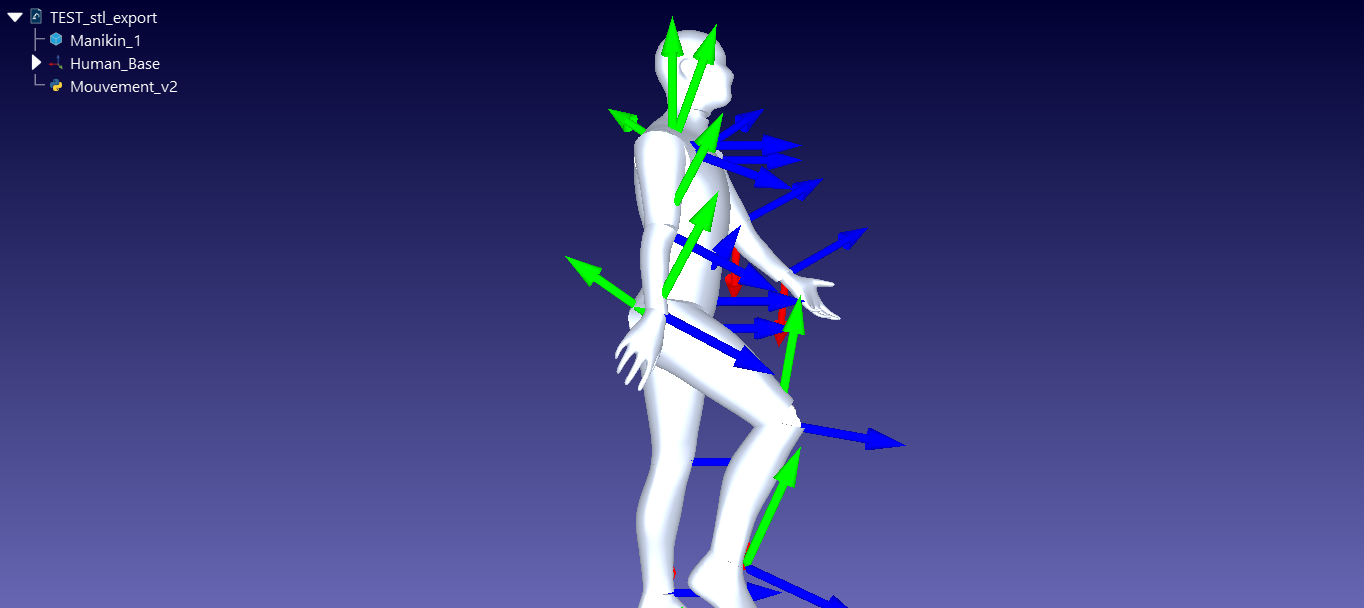
\includegraphics[width=0.46\textwidth]{marche_militaire.png}}\hfil
  \subfloat[Marche avant (profil)]{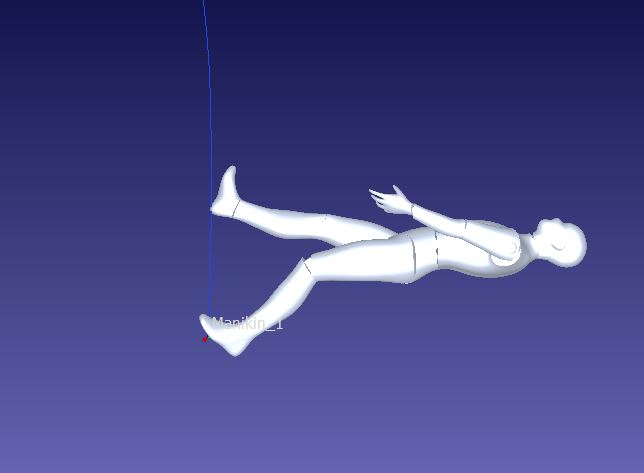
\includegraphics[width=0.46\textwidth]{marche_avant.jpg}}
  \caption{Les deux marches de base. La jambe d'appui reste tendue ; le balancier
  des bras est en opposition de phase.}
  \label{fig:marches}
\end{figure}

\begin{figure}[H]
  \centering
  \subfloat[Vue de dessus]{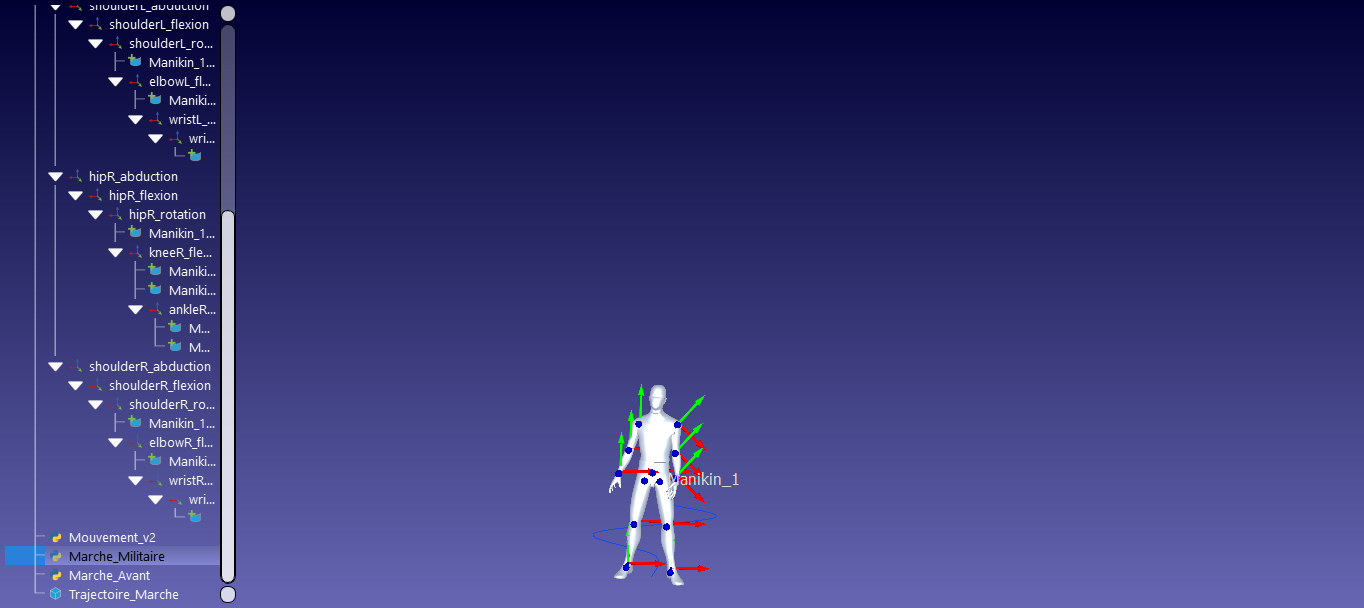
\includegraphics[width=0.46\textwidth]{traj_top.png}}\hfil
  \subfloat[Profil]{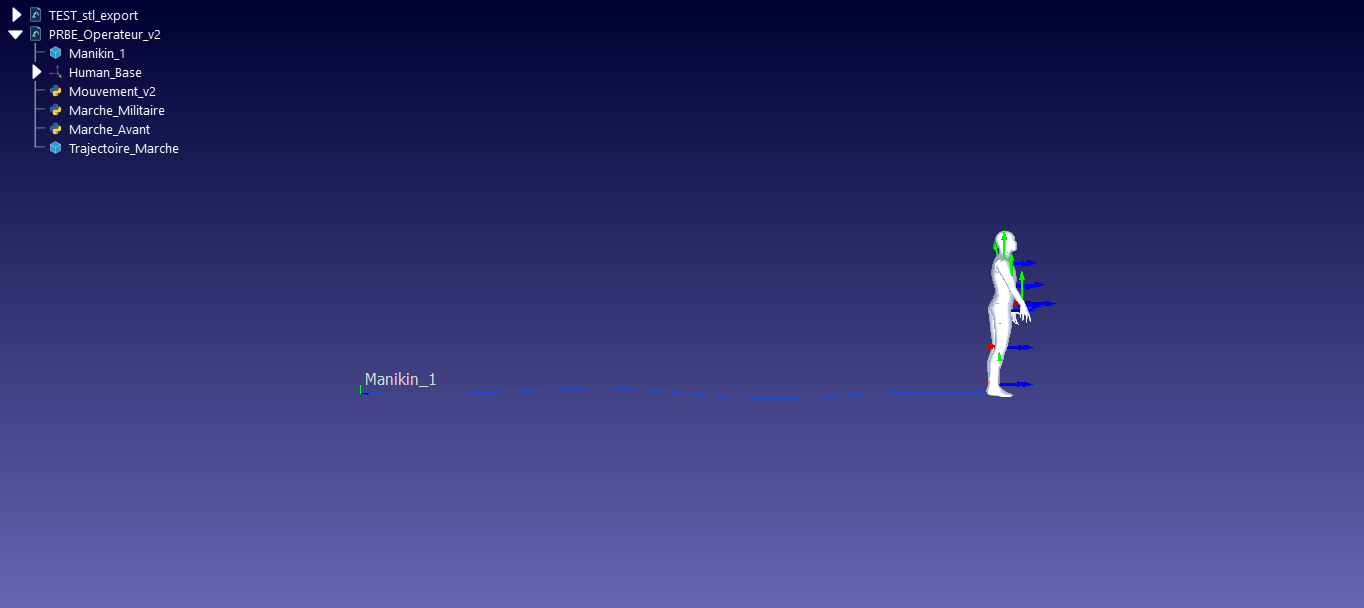
\includegraphics[width=0.46\textwidth]{traj_profil.png}}
  \caption{Marche sur trajectoire externe (spline en S) : la courbe (en bleu) est
  définie par des points dans un fichier, indépendamment du code d'animation.}
  \label{fig:traj}
\end{figure}

% ---------------------------------------------------------------
\subsection{Manipulation (membres supérieurs) : tâche du bras}
\label{ssec:bras}

La tâche de manipulation est un \emph{pick \& place} : le bras gauche (6~DDL) va
saisir une pièce cubique posée sur une table, la déplace et la repose, le reste du
corps restant fixe.

\paragraph{Cinématique inverse.} Atteindre la pièce avec la bonne orientation de
main est un problème de \textbf{cinématique inverse à 6~contraintes}
(position + orientation). On le résout par \emph{moindres carrés amortis}
(\emph{Damped Least Squares}). À chaque itération, l'erreur de pose
$\bm{e} = [\,\Delta\bm{p}\,;\,\Delta\bm{\theta}\,]$ (écart de position et
d'orientation) est réduite par
\[
\Delta \bm{q} = \bm{J}^{\!\top}\bigl(\bm{J}\bm{J}^{\!\top} + \lambda^2 \bm{I}\bigr)^{-1}\bm{e},
\]
où $\bm{J}$ est la jacobienne du bras (calculée par différences finies) et
$\lambda$ l'amortissement qui stabilise la convergence près des singularités. Une
\textbf{tâche posturale secondaire} oriente le choix de configuration : parmi les
solutions possibles, on privilégie celle où le \textbf{coude part en arrière}
(geste humain), jamais vers l'avant.

\paragraph{Trajectoire précalculée.} Pour un mouvement fluide, l'IK n'est résolue
qu'aux \textbf{poses clés} (saisie, transit, dépose), hors animation ; le bras lit
ensuite la trajectoire interpolée à cadence fixe. On évite ainsi des centaines de
résolutions par image : le geste complet dure environ $7$~s et reste régulier.

\paragraph{Position de la pièce externalisée.} Les coordonnées de la pièce sont des
\textbf{paramètres} du scénario, séparés du code de trajectoire : changer la
position de la cible suffit à faire que le bras aille la chercher ailleurs, sans
rien modifier d'autre (validé en \cref{sec:tests}).

\paragraph{Déroulé du geste.} Le mouvement enchaîne quatre temps, conçus pour
rester atteignables le coude en arrière (\cref{fig:bras}) : (1)~\emph{approche}
--- la main descend vers la pièce, paume orientée vers le bas ;
(2)~\emph{saisie} --- la pièce est solidarisée à la main ;
(3)~\emph{transit} --- le bras la déplace en restant proche du corps, la hauteur
de transit étant volontairement basse pour ne pas pousser le coude vers l'avant ;
(4)~\emph{dépose} --- la pièce est reposée à sa nouvelle position. Une micro-pause
sépare chaque temps pour stabiliser le geste.

\begin{figure}[H]
  \centering
  \subfloat[Approche]{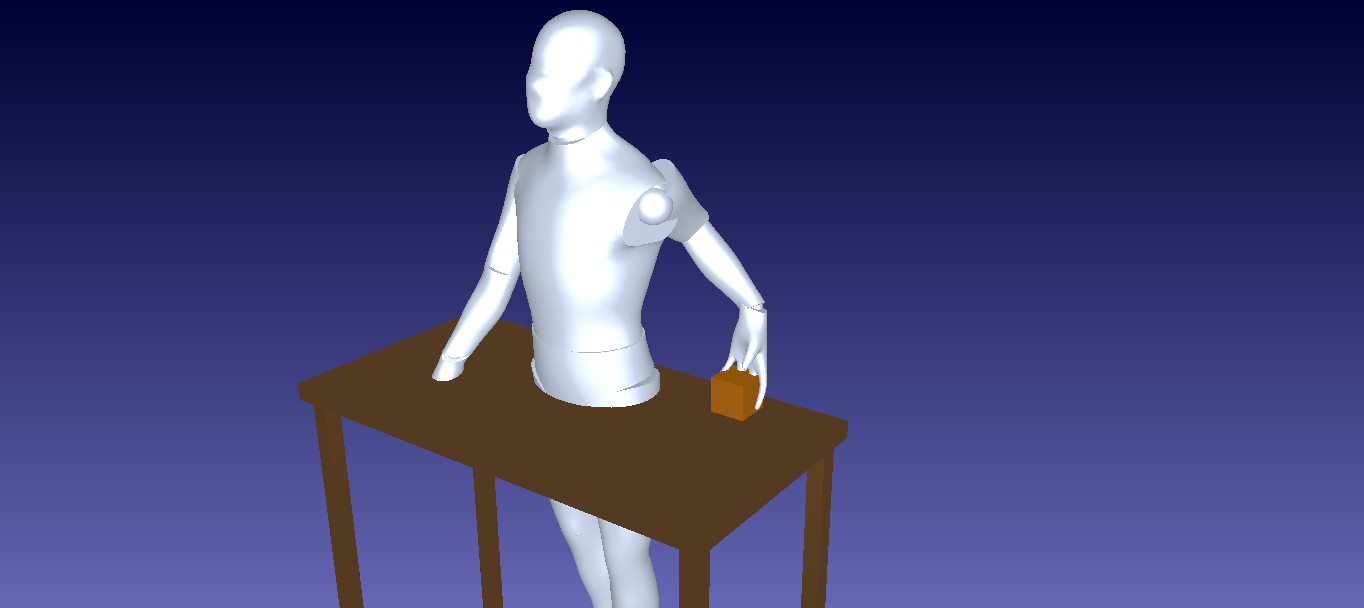
\includegraphics[width=0.23\textwidth]{bras_seq0.png}}\hfil
  \subfloat[Saisie]{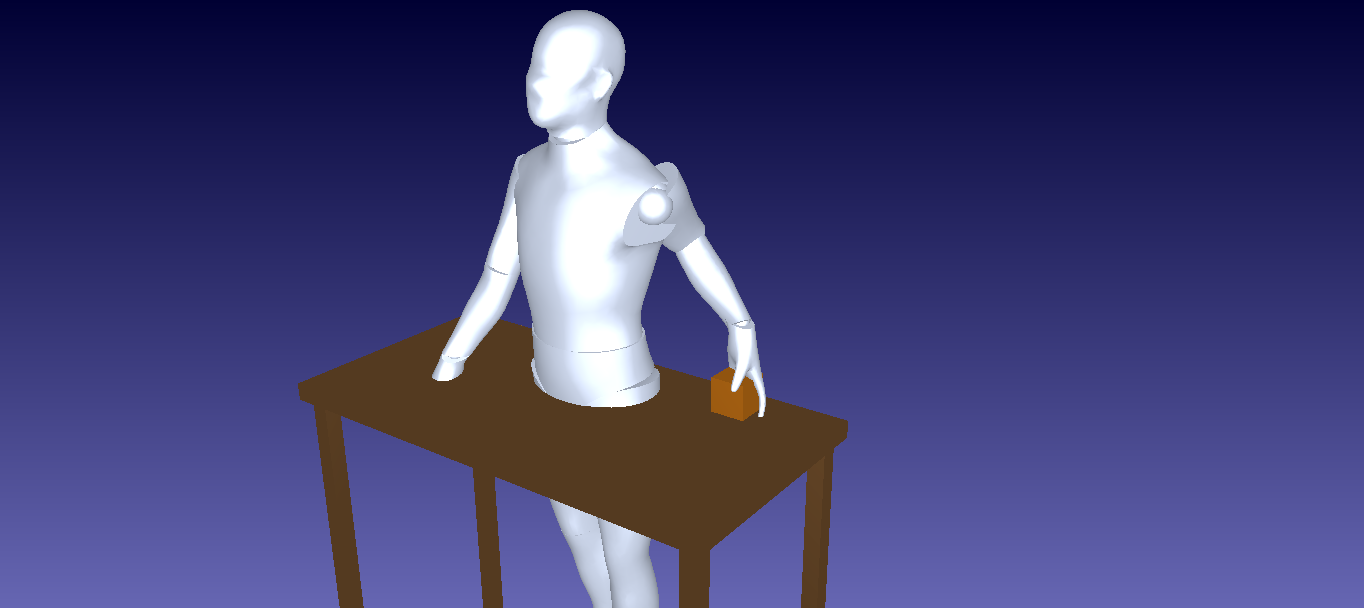
\includegraphics[width=0.23\textwidth]{bras_seq2.png}}\hfil
  \subfloat[Transit]{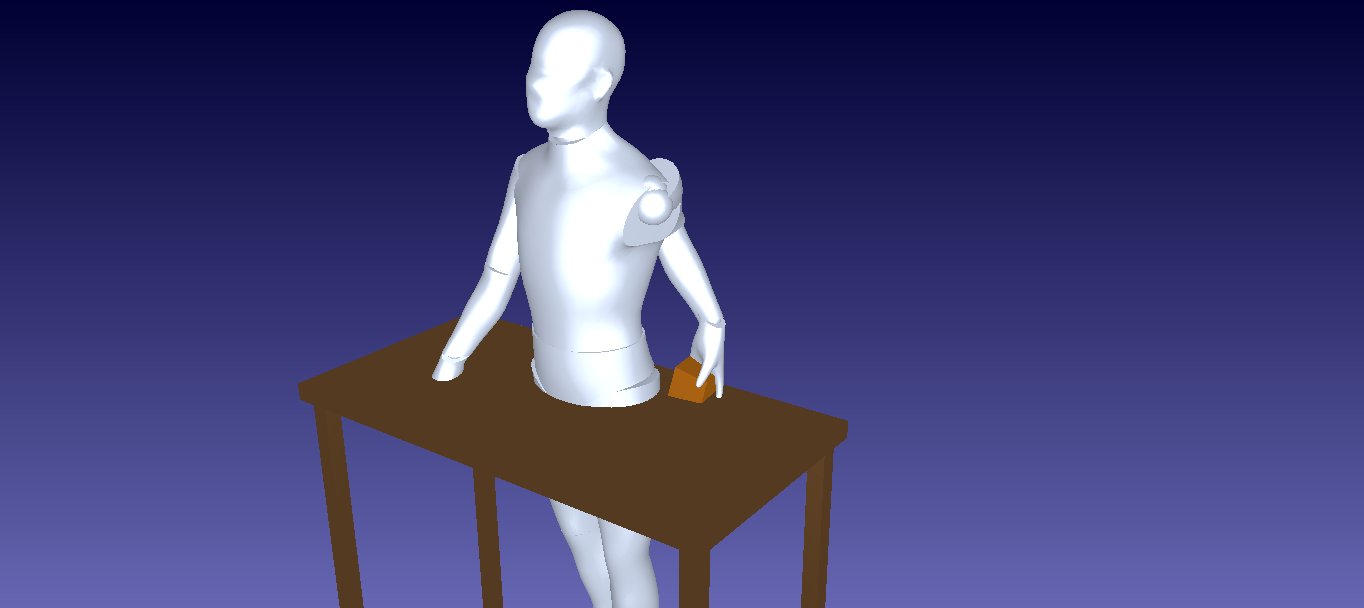
\includegraphics[width=0.23\textwidth]{bras_seq4.png}}\hfil
  \subfloat[Dépose]{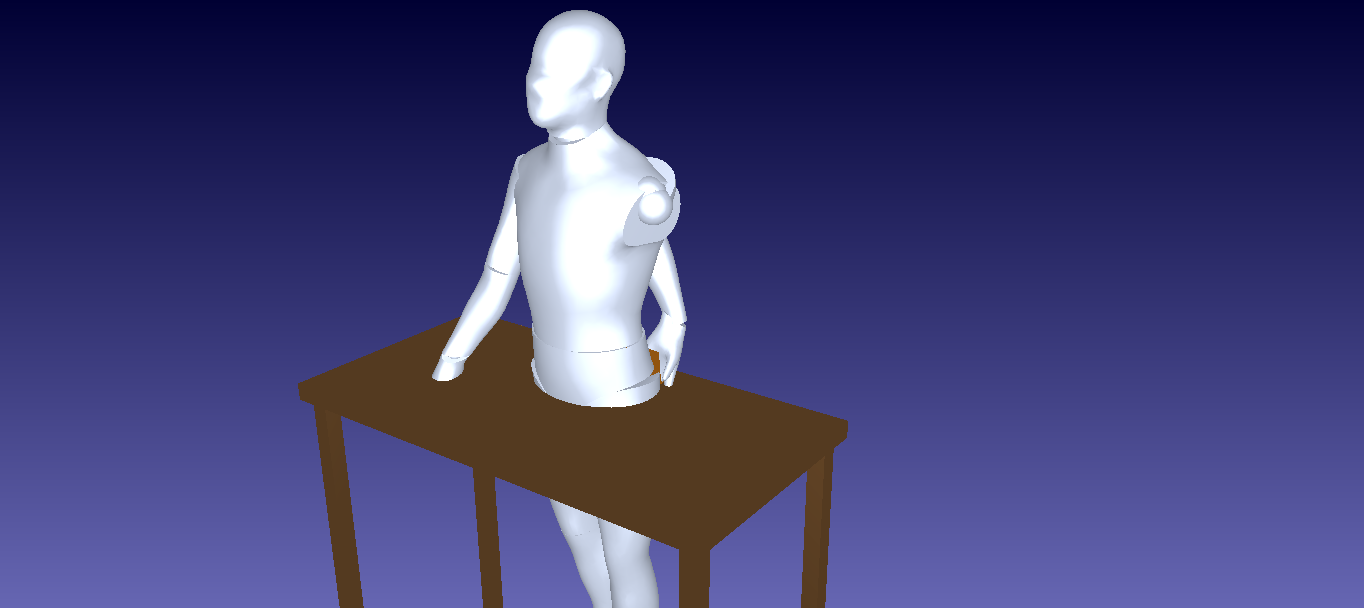
\includegraphics[width=0.23\textwidth]{bras_seq7.png}}
  \caption{Étapes du \emph{pick \& place} de la pièce cubique sur la table
  (tâche \texttt{Tache\_Bras.py}, bras gauche) : le coude reste en arrière
  pendant tout le geste.}
  \label{fig:bras}
\end{figure}

% =====================================================================
% SECTION 6 — TESTS ET RESULTATS                                [NIKO]
% Problemes identifies + corrections ; resolu (montre) vs perspective.
% =====================================================================

\rsection{Tests et résultats}
\label{sec:tests}

Le développement a été conduit de façon \emph{itérative}, chaque version étant
confrontée à un test objectif. Cette section présente les principaux problèmes
rencontrés, leur correction, et distingue ce qui est \textbf{résolu} de ce qui
reste \textbf{en perspective}.

% ---------------------------------------------------------------
\subsection{Persistance de la station : le mannequin « éclaté »}

\paragraph{Symptôme.} À la réouverture du fichier \texttt{.rdk}, le mannequin
apparaissait \emph{éclaté}, les segments dispersés alors que les repères restaient
en place.

\paragraph{Diagnostic.} Un outil de comparaison de poses (\emph{avant} sauvegarde /
\emph{après} réouverture) a montré que les repères, eux, survivent parfaitement.
La cause est que les sous-solides issus du \texttt{Split} sont des items d'un type
particulier (courbes) dont la pose relative \textbf{n'est pas persistée} : le
fichier sauvegarde leurs points bruts, et à l'ouverture la transformation du
parent est appliquée \emph{une seconde fois} --- d'où l'explosion. L'hypothèse
initiale (un repère de base désaligné) a ainsi été \textbf{écartée par la mesure}.

\paragraph{Correction.} Un script de ré-attachement recompose le mannequin en
$\approx 2$~s, sans reconstruction complète, en re-basant chaque segment sur son
repère. Il est embarqué dans la station (un double-clic après ouverture) et muni
d'un garde anti double-application. \textbf{Résultat : résolu} --- l'opérateur se
recompose à l'identique à chaque ouverture.

% ---------------------------------------------------------------
\subsection{Validation des mouvements}

\paragraph{Cohérence anatomique (branche d'IK).} Une articulation pivot admet deux
configurations symétriques ; la mauvaise donne un genou « à l'envers ». On force la
\textbf{branche anatomique} (genou et coude pliant dans le sens humain),
visualisée et fixée comme contrainte de posture (\cref{fig:branche}).

\begin{figure}[H]
  \centering
  \subfloat[Branche rejetée]{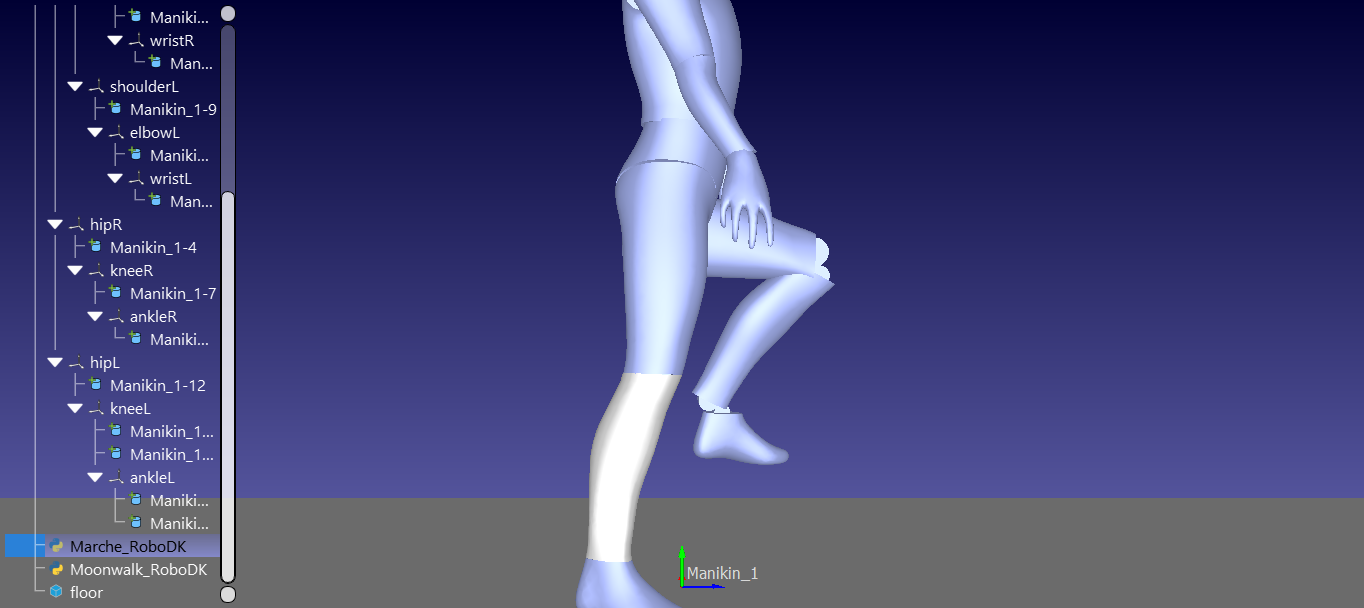
\includegraphics[width=0.46\textwidth]{knee_branche_A.png}}\hfil
  \subfloat[Branche retenue (sens humain)]{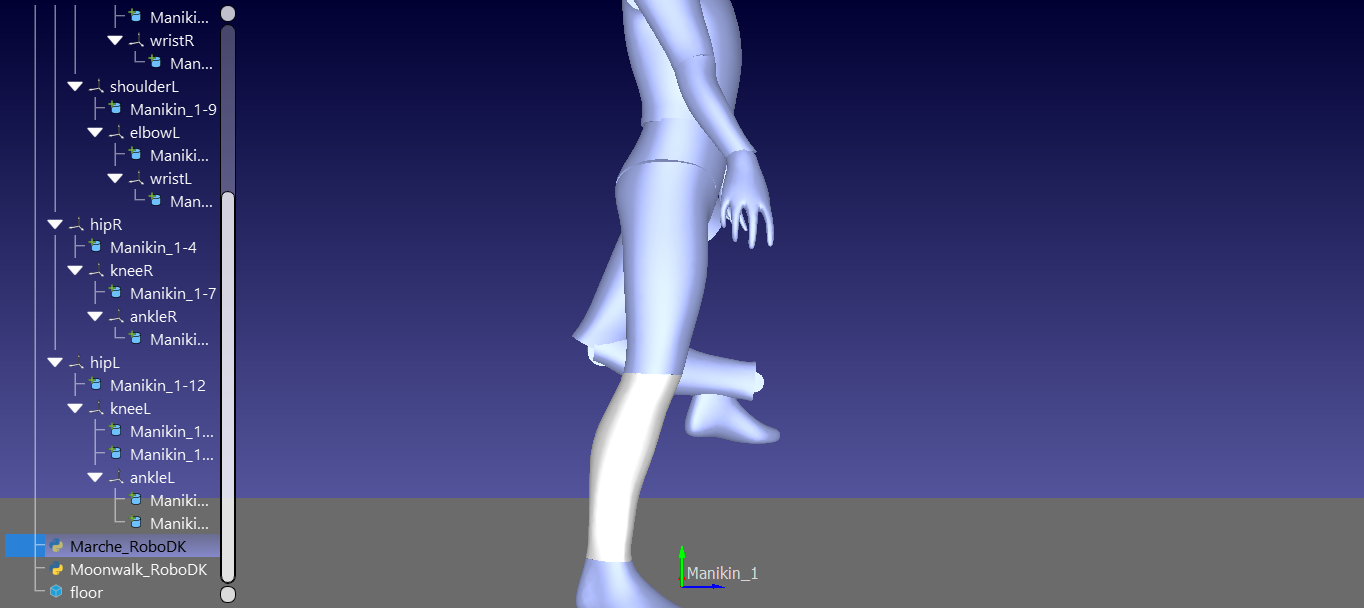
\includegraphics[width=0.46\textwidth]{knee_branche_B.png}}
  \caption{Sélection de la branche de flexion du genou : on impose la solution
  anatomiquement correcte.}
  \label{fig:branche}
\end{figure}

\paragraph{Non-collision.} Pour la tâche du bras, la validation ne se fait pas à
l'\oe il mais par \textbf{détection de collision sur les maillages} dans
\textsc{RoboDK} : le geste retenu présente \textbf{zéro collision} entre la main,
le corps et la table sur l'ensemble de la trajectoire. Une approximation
géométrique grossière (« doigts = paume $-115$~mm ») s'était au contraire révélée
insuffisante --- seul le maillage fait foi.

\paragraph{Reproductibilité.} Chaque animation laissait un résidu de quelques
degrés qui s'accumulait d'un essai à l'autre. Une remise au garde-à-vous exact,
appelée automatiquement avant chaque scénario, a supprimé cette dérive.

% ---------------------------------------------------------------
\subsection{Adaptation à la position de la pièce}

L'exigence d'\textbf{externaliser la position de la pièce} a été testée en
modifiant uniquement les coordonnées de la cible : le bras va chercher la pièce à
son nouvel emplacement et exécute le \emph{pick \& place} \textbf{sans aucune
modification du code de trajectoire}. \textbf{Résultat : résolu} (démonstration en
direct concluante).

% ---------------------------------------------------------------
\subsection{Problèmes ouverts et perspectives}

\begin{table}[H]
\centering
\caption{Synthèse : statut des points techniques.}
\label{tab:statut}
\small
\begin{tabularx}{\textwidth}{@{}p{5.2cm}cX@{}}
\toprule
\textbf{Point} & \textbf{Statut} & \textbf{Commentaire} \\
\midrule
Persistance du \texttt{.rdk} & \textcolor{supmerange}{Résolu} & Ré-attachement en $\approx 2$~s, embarqué \\
Branche d'IK (genou/coude) & \textcolor{supmerange}{Résolu} & Contrainte de posture anatomique \\
Non-collision (tâche bras) & \textcolor{supmerange}{Résolu} & 0 collision maillage sur la trajectoire \\
Position de pièce externalisée & \textcolor{supmerange}{Résolu} & Paramètre séparé, testé \\
DDL du poignet (pronation) & Perspective & Manque pour un geste pleinement naturel : à documenter, voire à ajouter \\
Collision arrière du coude & À surveiller & Direction correcte (coude en arrière), marge arrière à vérifier \\
Exécution hors-ligne & À vérifier & Confirmer l'absence de dépendances réseau \\
Intégration ligne ALIX & Perspective & Recentrer le \emph{human frame} et placer l'opérateur dans la cellule \\
\bottomrule
\end{tabularx}
\end{table}

% =====================================================================
% SECTION 7 — CONCLUSION ET PERSPECTIVES                        [NIKO]
% Revenir sur les objectifs annonces (atteints / non) + perspectives.
% =====================================================================

\rsection{Conclusion et perspectives}
\label{sec:conclusion}

Le projet visait à \textbf{lever un verrou} : faire vivre un opérateur humain
articulé à l'intérieur de \textsc{RoboDK}, là où le logiciel n'offre aucun modèle
humain pilotable. Ce pont a été construit.

\paragraph{Objectifs atteints.}
\begin{itemize}[noitemsep]
  \item \textbf{Modèle cinématique simplifié} --- un opérateur à \textbf{22~DDL}
        reconstruit dans \textsc{RoboDK} à partir d'un modèle 3D, sans import URDF
        ni \emph{Build Mechanism}, avec axes et butées anatomiques
        (\cref{sec:modele}).
  \item \textbf{Membres inférieurs} --- trois locomotions fonctionnelles : marche
        militaire, marche avant naturelle (anti-glissement), et marche guidée par
        une trajectoire externe (\cref{ssec:loco}).
  \item \textbf{Membres supérieurs} --- une tâche de manipulation \emph{pick \&
        place} par cinématique inverse, geste anatomique (coude en arrière) validé
        sans collision (\cref{ssec:bras}).
  \item \textbf{Robustesse} --- la station se recompose automatiquement et les
        animations sont reproductibles (\cref{sec:tests}).
\end{itemize}

\paragraph{Atteints partiellement.} La brique « opérateur » nécessaire aux
\textbf{scénarios d'interaction homme-robot} (coexistence, synchronisation) est
prête et paramétrable ; leur mise en scène complète sur la ligne ALIX et
l'\textbf{analyse sécurité/ergonomie} associée (distances normalisées, postures
tenables) constituent l'étape suivante.

\paragraph{Perspectives.}
\begin{itemize}[noitemsep]
  \item \textbf{Ajouter un DDL de poignet} (pronation de l'avant-bras) : son
        absence contraint certaines orientations de main --- limite identifiée et
        quantifiée.
  \item \textbf{Surveiller la collision arrière du coude} et affiner les marges du
        geste de manipulation.
  \item \textbf{Intégrer l'opérateur dans la cellule ALIX} (recentrage du
        \emph{human frame}) et le \textbf{tester sur le robot réel}, avec captures
        vidéo.
  \item \textbf{Fiabiliser la persistance} de la station (au-delà du
        ré-attachement) et \textbf{confirmer l'exécution hors-ligne}.
\end{itemize}

\medskip
Au-delà des livrables, le projet a montré qu'une \textbf{démarche outillée et
itérative} --- mesurer avant de conclure, valider par la collision plutôt qu'à
l'\oe il, externaliser les paramètres --- permet d'obtenir un modèle humain
crédible et réutilisable dans un simulateur qui n'y était pas destiné.

% ====================== ANNEXES ======================
\newpage
\appendix
\rsection{Cahier des charges complet}
\label{annexe:cdc}

La version complète du cahier des charges (scénarios détaillés, exigences
fonctionnelles exhaustives, périmètre et limites, planning) est maintenue dans le
dépôt GitHub du projet et n'est pas reproduite intégralement ici afin de garder le
rapport concis (la qualité primant sur la quantité).

{\sloppy
\begin{itemize}[noitemsep]
  \item Dépôt : \url{https://github.com/ProjectInitNiko/PRBE-Homme-Robot}
  \item Document : \texttt{docs/cahier-des-charges.md} (version Markdown) et
        \texttt{docs/PRBE-Cahier\_des\_charges.pdf} (version PDF, 17~p.).
\end{itemize}\par}

% ====================== BIBLIOGRAPHIE ======================
\newpage
\barre\par\vspace{2pt}
\addcontentsline{toc}{section}{Références}
\bibliography{references}

\end{document}
